%%%%%%%%%%%%%%%%%%%%%%%%%%%%%%%%%%%%%%%%%%%%%%%%%%%%%%%%%%%%%%%%%%%%%%%%%%%%%%%%%%%%%%%%%%%%%%%
%% Description:       Programmentwurf advanced software engineering
%% Author:      Manuel Berg, m.berg@enbw.com
%%  -*- coding: utf-8 -*-
%%%%%%%%%%%%%%%%%%%%%%%%%%%%%%%%%%%%%%%%%%%%%%%%%%%%%%%%%%%%%%%%%%%%%%%%%%%%%%%%%%%%%%%%%%%%%%%

\titlespacing*{\chapter}{0pt}{-30mm}{10pt}
\titleformat{\chapter}[display]
  {\normalfont\bfseries}{}{10pt}{\Huge\thechapter.\quad}
  
\chapter{Clean Architecture (8P)}
\pagestyle{scrheadings}
\clearscrheadfoot
\pagenumbering{arabic}
\setcounter{page}{3}
\ofoot[\pagemark]{\pagemark}
%\ohead[\headmark]{\headmark}
\onehalfspacing

\section{Was ist Clean Architecture? (1P)}
\emph{[Allgemeine Beschreibung der Clean Architecture in eigenen Worten]}
\\
\\
\noindent Unter der \emph{Clean Architecture} versteht man eine Architekturrichtlinie. Die Grundidee kann man sich als eine Zwiebel vorstellen, welche aus fünf Schichten besteht. Die fünf Schichten Plugins, Adapters, Application Code, Domain Code sowie Abstraction Code stellen hierbei die Bereiche der Software dar. So bildet der Abstraction Code den innersten Kern, und die Plugins bilden die äußerste Hülle. Je weiter ein Ring vom Kern entfernt ist, desto \enquote{sichtbarer} ist er in der tatsächlichen Anwendung und desto mehr Änderungen erfährt er.

Ein zentraler Aspekt der \emph{Clean Architecture} ist hierbei die sogenannte \emph{Dependency Rule}. Diese besagt, dass Abhängigkeiten in dem zuvor erwähnten Modell nur nach Innen -- also in Richtung des Kerns (Abstraction Code) -- zeigen dürfen. So darf die Adapters-Schicht beispielsweise von der Schicht des Application Codes abhängig sein, jedoch nicht von den Plugins.

\section{Analyse der Dependency Rule (2P)}
\emph{[1 Klasse, die die Dependency Rule einhält und 1 Klasse, die die Dependency Rule verletzt; jeweils
UML der Klasse und Analyse der Abhängigkeiten in beide Richtungen (d.h., von wem hängt die Klasse
ab und wer hängt von der Klasse ab) in Bezug auf die Dependency Rule]}

\subsubsection{Positiv-Beispiel: Dependency Rule}
\noindent Die Klasse \emph{Graph} befindet sich in der Domain Code-Schicht und realisiert die Knoten und Kanten des Spielfeldes. Da dies nur die Struktur des Spielfeldes enthält und in keinster Weise mit Spielständen zu tun hat, sind keine Abhängigkeiten in Richtung äußerer Schichten enthalten.

\newpage
\noindent
\begin{figure}[htbp]
\centering
\centerline{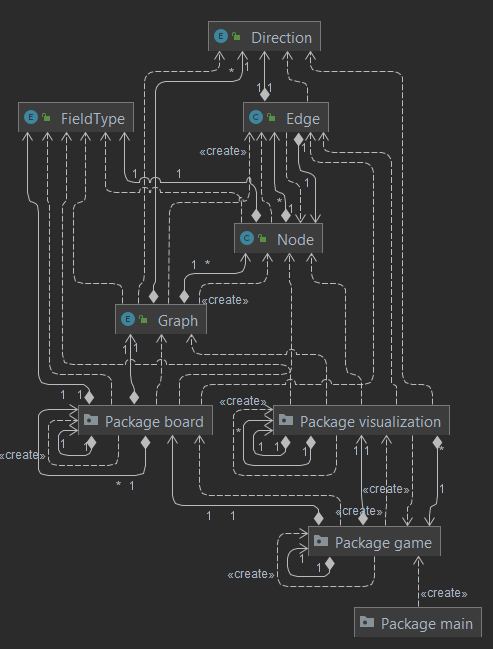
\includegraphics[scale=.5]{dependencyrule_klasse_graph}}
\caption{Positiv-Beispiel Dependency Rule [Eigene Darstellung aus \emph{IntelliJ}]}
\label{fig:dependencyrulepositiv}
\end{figure}
\\
\noindent In der \hyperref[fig:dependencyrulepositiv]{Abbildung 2.1} sind alle sichtbaren Klassen in derselben Schicht wie die \emph{Graph}-Klasse. Die in den Packages enthaltenen Klassen wiederum befinden sich in anderen Schichten. Da es von der \emph{Graph}-Klasse keine Abhängigkeit auf eines der anderen Packages (und somit auch nicht auf andere Schichten) gibt, ist dies ein Positivbeispiel für die Einhaltung der Dependency Rule.

\newpage
\noindent

\subsubsection{Negativ-Beispiel: Dependency Rule}
\noindent Bei der Klasse \emph{GameService} handelt es sich um Application Code, denn die Klasse kümmert sich um einen reibungslosen Spielablauf. Deshalb sollten hier auch grundsätzlich keine Abhängigkeiten auf die \acs{GUI} vorhanden sein.

\begin{figure}[htbp]
\centering
\centerline{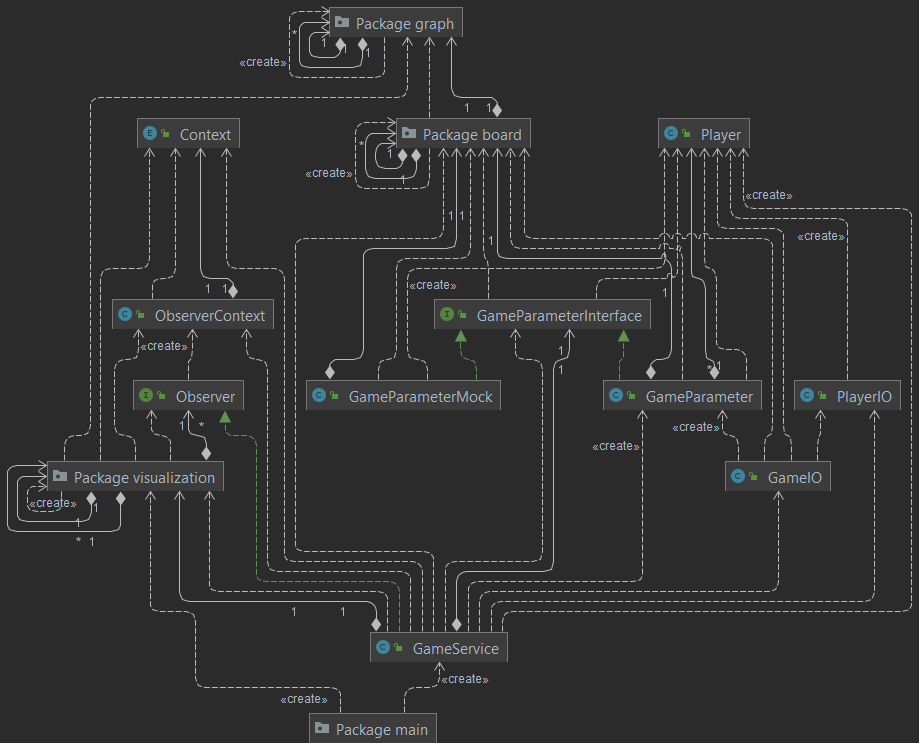
\includegraphics[scale=.5]{dependencyrule_klasse_gameservice}}
\caption{Negativ-Beispiel Dependency Rule [Eigene Darstellung aus \emph{IntelliJ}]}
\label{fig:dependencyrulenegativ}
\end{figure}

\noindent In \hyperref[fig:dependencyrulepositiv]{Abbildung 2.2} ist zu erkennen, dass die \emph{GameService}-Klasse Abhängigkeiten in Richtung der Klassen des Packages \emph{visualization} aufweist. Die Klassen dieses Packages sind verantwortlich für die \acs{GUI} und gehören somit zu äußersten Schicht. Aus diesem Grund liegt hier ein Negativ-Beispiel vor.

\newpage

\section{Analyse der Schichten (5P)}
\emph{[jeweils 1 Klasse zu 2 unterschiedlichen Schichten der Clean-Architecture: jeweils UML der Klasse
(ggf. auch zusammenspielenden Klassen), Beschreibung der Aufgabe, Einordnung mit Begründung in
die Clean-Architecture]}

\subsubsection{Schicht: Domain Code}
\begin{figure}[htbp]
\centering
\centerline{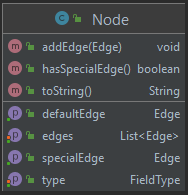
\includegraphics[scale=.35]{node}}
\caption{Klasse der Domain Code-Schicht [Eigene Darstellung aus \emph{IntelliJ}]}
\label{fig:klassedomaincodeschicht}
\end{figure}
\noindent Die Klasse \emph{Node} entspricht einem Spielfeld bei \emph{Mensch ärgere Dich nicht}. Jedes Feld, welches von einer Spielfigur besetzt werden kann, wird durch diese Klasse einem Feldtypen zugeordnet. Dies kann beispielsweise ein rotes Zielfeld oder auch ein grünes Startfeld sein. Außerdem enthält die Klasse eine Liste von Kanten, die ausgehend von diesem Knoten eine Verbindung zu einem anderen Knoten darstellen. In \hyperref[fig:klasseadomaincodeschicht]{obiger Abbildung} ist auch zu sehen, dass es Standardkanten und Spezialkanten gibt. Erstere können durch jede Spielfigur unabhängig von der Farbe befahren werden. Die Spezialkanten wiederum sind nur durch eine spezielle Farbe nutzbar. Das sind die vier Kanten, die zu den Zielfeldern zeigen.

Die Klasse \emph{Node} gehört zum inneren Kern der Anwendung und ist unabhängig vom Spielbetrieb. Die grundlegende Logik hinter dem Spielbrett mit den genannten Knoten und Kanten ändert sich nie. Gemäß den Vorlesungsinhalten handelt es sich deshalb um ein Teil der Domain Code-Schicht.
\newpage
\subsubsection{Schicht: Application Code}
\begin{figure}[htbp]
\centering
\centerline{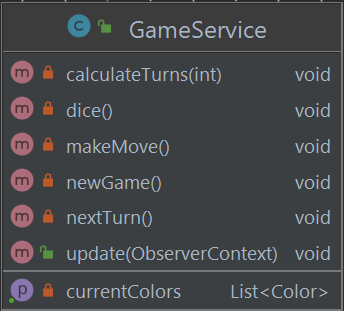
\includegraphics[scale=.42]{gameservice}}
\caption{Klasse der Application Code-Schicht [Eigene Darstellung aus \emph{IntelliJ}]}
\label{fig:klasseapplicationcodeschicht}
\end{figure}
\noindent Die Klasse \emph{GameService} kümmert sich um das Spielgeschehen. Dabei weiß sie um die aktuell am Spiel teilnehmenden Farben. Die Klasse kann ausgeben, wo sich eine Spielfigur nach einer gegebenen Augenzahl durch Würfeln befindet. Außerdem führt sie den Prozess des Würfelns durch Generierung von Zufallszahlen aus. Auch kann sie einen Zug durchführen, ein neues Spiel starten und bestimmen, welcher Spieler gerade an der Reihe ist. Die Klasse ist an der Implementierung des Observer-Patterns beteiligt. Sie reagiert dadurch auf Änderungen in der \acs{GUI}.

Die im vorherigen Abschnitt genannten Funktionen entsprechen anwendungsspezifischer Geschäftslogik. Deswegen wird dieser Klasse der Application Code-Schicht zugeordnet.